%%%%%%%%%%%%%%%%%%%%%%%%%%%%%%%%%%%%%%%%%
% Beamer Presentation
% LaTeX Template
% Version 1.0 (10/11/12)
%
% This template has been downloaded from:
% http://www.LaTeXTemplates.com
%
% License:
% CC BY-NC-SA 3.0 (http://creativecommons.org/licenses/by-nc-sa/3.0/)
%
%%%%%%%%%%%%%%%%%%%%%%%%%%%%%%%%%%%%%%%%%

%----------------------------------------------------------------------------------------
%	PACKAGES AND THEMES
%----------------------------------------------------------------------------------------

\documentclass{beamer}

\mode<presentation> {

% The Beamer class comes with a number of default slide themes
% which change the colors and layouts of slides. Below this is a list
% of all the themes, uncomment each in turn to see what they look like.

%\usetheme{default}
%\usetheme{AnnArbor}
%\usetheme{Antibes}
%\usetheme{Bergen}
%\usetheme{Berkeley}
%\usetheme{Berlin}
%\usetheme{Boadilla}
%\usetheme{CambridgeUS}
%\usetheme{Copenhagen}
%\usetheme{Darmstadt}
%\usetheme{Dresden}
%\usetheme{Frankfurt}
%\usetheme{Goettingen}
%\usetheme{Hannover}
%\usetheme{Ilmenau}
%\usetheme{JuanLesPins}
%\usetheme{Luebeck}
\usetheme{Madrid}
%\usetheme{Malmoe}
%\usetheme{Marburg}
%\usetheme{Montpellier}
%\usetheme{PaloAlto}
%\usetheme{Pittsburgh}
%\usetheme{Rochester}
%\usetheme{Singapore}
%\usetheme{Szeged}
%\usetheme{Warsaw}

% As well as themes, the Beamer class has a number of color themes
% for any slide theme. Uncomment each of these in turn to see how it
% changes the colors of your current slide theme.

%\usecolortheme{albatross}
%\usecolortheme{beaver}
%\usecolortheme{beetle}
%\usecolortheme{crane}
%\usecolortheme{dolphin}
%\usecolortheme{dove}
%\usecolortheme{fly}
%\usecolortheme{lily}
%\usecolortheme{orchid}
%\usecolortheme{rose}
%\usecolortheme{seagull}
%\usecolortheme{seahorse}
\usecolortheme{whale}
%\usecolortheme{wolverine}

\setbeamertemplate{footline} % To remove the footer line in all slides uncomment this line
%\setbeamertemplate{footline}[page number] % To replace the footer line in all slides with a simple slide count uncomment this line

\setbeamertemplate{navigation symbols}{} % To remove the navigation symbols from the bottom of all slides uncomment this line

}

\usepackage{graphicx} % Allows including images
\usepackage{booktabs} % Allows the use of \toprule, \midrule and \bottomrule in tables
\usepackage{sansmathaccent}

\pdfmapfile{+sansmathaccent.map}
\usepackage[plain]{algorithm}
\usepackage{algorithmicx}
\usepackage[noend]{algpseudocode}
\usepackage{listings}
\newcommand{\pseudoli}[1]{\lstinline[style=pseudo]!#1!}
% Deprecated Environments (Replaced by Algorithmic package)
\lstdefinestyle{pseudo}{basicstyle=\rmfamily,
                        upquote=true,
                        keywordstyle=\color{black}\bfseries,
                        commentstyle=\color[rgb]{0.133,0.545,0.133},
                        stringstyle=\color[rgb]{0.627,0.126,0.941},}
\usepackage{ulem}
\renewcommand<>{\sout}[1]{
\alt#2{\beameroriginal{\sout}{#1}}{#1}
}
\usepackage{tikz}
\usetikzlibrary{trees, arrows, decorations}
%----------------------------------------------------------------------------------------
%	TITLE PAGE
%----------------------------------------------------------------------------------------

\title[Algorithms 1]{Greedy Algorithms 1} % The short title appears at the bottom of every slide, the full title is only on the title page

%\author{John Smith} % Your name
\institute[BYU] % Your institution as it will appear on the bottom of every slide, may be shorthand to save space
{
Brigham Young University \\ % Your institution for the title page
\medskip
%\textit{john@smith.com} % Your email address
}
\date{\today} % Date, can be changed to a custom date

\begin{document}

\begin{frame}
\titlepage % Print the title page as the first slide
\end{frame}

%\begin{frame}
%\frametitle{Overview} % Table of contents slide, comment this block out to remove it
%\tableofcontents % Throughout your presentation, if you choose to use \section{} and %\subsection{} commands, these will automatically be printed on this slide as an overview of your presentation
%\end{frame}

%----------------------------------------------------------------------------------------
%	PRESENTATION SLIDES
%----------------------------------------------------------------------------------------

%------------------------------------------------
%\section{First Section} % Sections can be created in order to organize your presentation into %discrete blocks, all sections and subsections are automatically printed in the table of contents %as an overview of the talk
%------------------------------------------------

%\subsection{Subsection Example} % A subsection can be created just before a set of slides with %a common theme to further break down your presentation into chunks

%\begin{frame}
%\frametitle{AVL trees}
%Sed iaculis dapibus gravida. Morbi sed tortor erat, nec interdum arcu. Sed id lorem lectus. %Quisque viverra augue id sem ornare non aliquam nibh tristique. Aenean in ligula nisl. Nulla sed %tellus ipsum. Donec vestibulum ligula non lorem vulputate fermentum accumsan neque mollis.%\\~\\

%Sed diam enim, sagittis nec condimentum sit amet, ullamcorper sit amet libero. Aliquam vel dui %orci, a porta odio. Nullam id suscipit ipsum. Aenean lobortis commodo sem, ut commodo leo %gravida vitae. Pellentesque vehicula ante iaculis arcu pretium rutrum eget sit amet purus. %Integer ornare nulla quis neque ultrices lobortis. Vestibulum ultrices tincidunt libero, quis %commodo erat ullamcorper id.
%\end{frame}

%------------------------------------------------

%------------------------------------------------
%greedy Algorithms
\begin{frame}
\frametitle{Greedy Algorithms}
\begin{itemize}
\item A \textbf{greedy algorithm} is incrementally optimal - at each step it goes for whatever is best.
\item They are easy to understand and program, but often will miss the best possible outcome.
\end{itemize}
\end{frame}
%-----------------------------------------------
\begin{frame}
\frametitle{Example}
\begin{center}
Maximize payoff by traversing the tree from the root to a leaf.
\end{center}

\begin{columns}[c]
\column{.5\textwidth}
\begin{center}

\begin{tikzpicture}[
  level distance=1.5 cm,
  level 1/.style={sibling distance=3cm},
  level 2/.style={sibling distance=1.5cm},
   thick]
 \pgfdeclaredecoration{sl}{initial}{
  \state{initial}[width=\pgfdecoratedpathlength-1sp]{
     \pgfmoveto{\pgfpointorigin}
  }
  \state{final}{
     \pgflineto{\pgfpointorigin}
    }
}
\only<1-2>{
\tikzset{parallel arrow/.style={->, 
     shorten >=2mm, shorten <=2mm, 
     decoration={sl,raise=-.2cm}, blue!40!cyan, decorate}}
     }
\only<3->{
\tikzset{parallel arrow/.style={->, 
     shorten >=2mm, shorten <=2mm, 
     decoration={sl,raise=.2cm}, blue!40!cyan, decorate}}
     % change raise to .2cm
}
\tikzset{edge label/.style={
        font=\tiny,
        auto=right,
        ellipse,inner sep=1.75mm,
    }
} 


  \node[circle,draw](1) {1}
	child {node[circle,draw](2){2}
		child{node[circle,draw](4){4}
			edge from parent node[left]{99}
		}
		child{node[circle,draw](5){5}
			edge from parent node[right]{6}
		}
		edge from parent node[left]{4}
	}
	child{node[circle,draw](3){3}
		child{node[circle,draw](6){6}
			edge from parent node [left]{20}
		}
		child{node[circle,draw](7){7}
			edge from parent node[right]{40}
		}
		edge from parent node[right]{20}
	};
\only<2>{
\foreach \s/\t/\i in {1/3/, 3/7/} {
   \draw[] (\s) edge[parallel arrow](\t);}
   }
\only<3>{
\foreach \s/\t/\i in {1/2/, 2/4/} {
   \draw[] (\s) edge[parallel arrow](\t);}%%%%%%%%%%%%%% Fix arrows
   }
\end{tikzpicture}

\end{center}
\column{.5\textwidth}
\begin{itemize}
\item Choose the path with the highest value at each step.
\item \pause $1, 3, 7$ gets $60$.
\item \pause But maximum path is $1, 2, 4$ with a value of $103$.
\end{itemize}
\end{columns}
\end{frame}

%-----------------------------------------------
% MST
\begin{frame}
\frametitle{Minimum Spanning Tree}
\begin{itemize}
\item A graph's \textbf{spanning tree} is a subgraph that is a tree and contains all of the vertices.
\item A \textbf{minimum spanning tree} or \textbf{MST} is the spanning tree that minimizes the total weight.
\item A graph may have many possible spanning trees and MSTs.
\end{itemize}
\begin{columns}[c]
\column{.3\textwidth}
\begin{center}

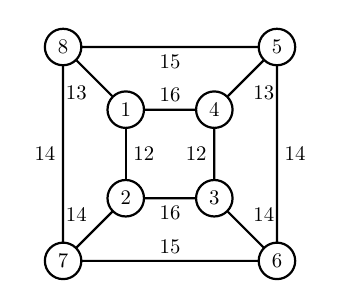
\begin{tikzpicture}[scale=.75, transform shape, auto,node distance=1.5cm,
 thick,main node/.style={circle,draw}]
 
  \node[main node] (1) [] {1};
  \node[main node] (2) [below of=1] {2};
  \node[main node] (3) [right of=2] {3};
  \node[main node] (4) [above of=3] {4};
  \node[main node] (5) [above right of=4] {5};  
  \node[main node] (6) [below right of=3] {6};
  \node[main node] (7) [below left of=2] {7};
  \node[main node] (8) [above left of=1] {8};
  
  \foreach \s/\t/\i in {1/2/12, 1/4/16, 1/8/13, 3/2/16, 3/4/12, 3/6/14, 5/4/13, 5/6/14, 5/8/15, 7/2/14, 7/6/15, 7/8/14} {
   \path[draw] (\s) edge node {\i} (\t);}
\end{tikzpicture}

Graph

\end{center}
\column{.3\textwidth}
\begin{center}

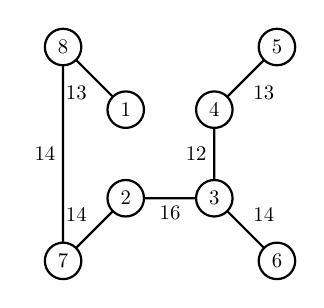
\begin{tikzpicture}[scale=.75, transform shape,auto,node distance=1.5cm,
 thick,main node/.style={circle,draw}]
 
  \node[main node] (1) [] {1};
  \node[main node] (2) [below of=1] {2};
  \node[main node] (3) [right of=2] {3};
  \node[main node] (4) [above of=3] {4};
  \node[main node] (5) [above right of=4] {5};  
  \node[main node] (6) [below right of=3] {6};
  \node[main node] (7) [below left of=2] {7};
  \node[main node] (8) [above left of=1] {8};
 
  \foreach \s/\t/\i in {7/8/14, 7/2/14, 3/4/12, 3/6/14, 5/4/13, 3/2/16, 1/8/13} {
   \path[draw] (\s) edge node {\i} (\t);}
 \end{tikzpicture}

A spanning tree with total weight 96

\end{center}
\column{.3\textwidth}
\begin{center}

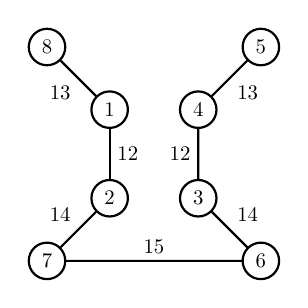
\begin{tikzpicture}[scale=.75, transform shape,auto,node distance=1.5cm,
 thick,main node/.style={circle,draw}]
 
  \node[main node] (1) [] {1};
  \node[main node] (2) [below of=1] {2};
  \node[main node] (3) [right of=2] {3};
  \node[main node] (4) [above of=3] {4};
  \node[main node] (5) [above right of=4] {5};  
  \node[main node] (6) [below right of=3] {6};
  \node[main node] (7) [below left of=2] {7};
  \node[main node] (8) [above left of=1] {8};

  \foreach \s/\t/\i in {1/2/12, 7/2/14, 3/4/12, 3/6/14, 5/4/13, 7/6/15, 1/8/13} {
   \path[draw] (\s) edge node {\i} (\t);}  	 
\end{tikzpicture}

A MST with total weight 93

\end{center}
\end{columns}
\end{frame}

%----------------------------------------------
\begin{frame}
\frametitle{MST Applications}
\begin{itemize}
\item MSTs are used for network design.
\item This includes planning electric, power, sewer, phone, or water systems.
\item For example, laying down telephone wires costs money, but once connected the length of the wire does not affect the phone call.
\item A MST would tell the cheapest way to connect everyone with telephone wires.
\end{itemize}
\end{frame}

%----------------------------------------------
\begin{frame}
\frametitle{Making a MST}
\begin{itemize}
\item 2 ways of building a MST.
\item Kruskal's algorithm starts with a forest and grows until it becomes a tree.
\item Prim's algorithms is always a tree, and grows until it includes all the nodes.
\end{itemize}
\end{frame}
%----------------------------------------------
%Kruskals
\begin{frame}
\frametitle{Kruskal's Algorithm}
\begin{itemize}
\item List the edges in ascending order by weight.
\item Go through list, add in an edge if it won't make a cycle.
\item stop when you have $n-1$ edges, where $n$ is the number of nodes.
\item This is a greedy, because at each step we add the edge with the least weight.
\end{itemize}
\end{frame}
%------------------------------------------------
\begin{frame}
\frametitle{Kruskal Example}
\begin{center}
\only<1-7>{Walk through the list and add an edge if it doesn't create a cycle.}
\only<8> {(7,8) would create a cycle.}
\only<9> {(5,6) would create a cycle.}
\only<10> {Adding (5,8) makes all the nodes connected, so we are done.}
\end{center}
\begin{columns}[c]
\column{.4\textwidth}
\begin{center}
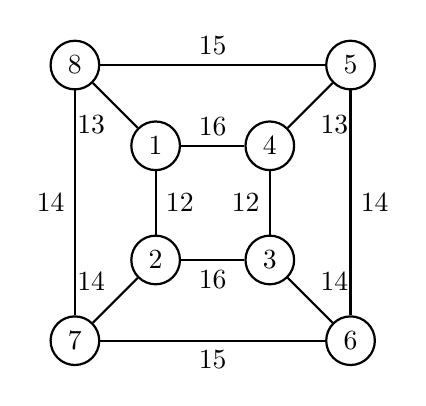
\begin{tikzpicture}[auto,node distance=1.45cm,
 thick,main node/.style={circle,draw}]
 
  \node[main node] (1) [] {1};
  \node[main node] (2) [below of=1] {2};
  \node[main node] (3) [right of=2] {3};
  \node[main node] (4) [above of=3] {4};
  \node[main node] (5) [above right of=4] {5};  
  \node[main node] (6) [below right of=3] {6};
  \node[main node] (7) [below left of=2] {7};
  \node[main node] (8) [above left of=1] {8};
  
  \foreach \s/\t/\i in {1/2/12, 1/4/16, 1/8/13, 3/2/16, 3/4/12, 3/6/14, 5/4/13, 5/6/14, 8/5/15, 7/2/14, 6/7/15, 7/8/14} {
   \path[draw] (\s) edge node {\i} (\t);}
\end{tikzpicture}
\end{center}
\column{.2\textwidth}

\begin{tabular}{|c|c|}
\hline
\textbf<2>{(1,2)} & 12 \\
\textbf<3>{(3,4)} & 12 \\
\textbf<4>{(1,8)} & 13 \\
\textbf<5>{(4,5)} & 13 \\
\textbf<6>{(2,7)} & 14 \\
\textbf<7>{(3,6)} & 14 \\
\textbf<8>{\sout<8->{(7,8)}} & 14 \\
\textbf<9>{\sout<9->{(5,6)}} & 14 \\
\textbf<10>{(5,8)} & 15 \\
(6,7) & 15 \\
(1,4) & 16 \\
\hline
\end{tabular}

\column{.4\textwidth}
\begin{center}

\begin{tikzpicture}[auto,node distance=1.45cm,
 thick,main node/.style={circle,draw}]
 
  \node[main node] (1) [] {1};
  \node[main node] (2) [below of=1] {2};
  \node[main node] (3) [right of=2] {3};
  \node[main node] (4) [above of=3] {4};
  \node[main node] (5) [above right of=4] {5};  
  \node[main node] (6) [below right of=3] {6};
  \node[main node] (7) [below left of=2] {7};
  \node[main node] (8) [above left of=1] {8};

  \only<2->{
   \foreach \s/\t/\i in {1/2/12} {
   \path[draw] (\s) edge node {\i} (\t);}
 }
 \only<3->{
   \foreach \s/\t/\i in {3/4/12} {
   \path[draw] (\s) edge node {\i} (\t);}
 }
 \only<4->{
   \foreach \s/\t/\i in {1/8/13} {
   \path[draw] (\s) edge node {\i} (\t);}
 }
 \only<5->{
   \foreach \s/\t/\i in {5/4/13} {
   \path[draw] (\s) edge node {\i} (\t);}
 }
 \only<6->{
   \foreach \s/\t/\i in {7/2/14} {
   \path[draw] (\s) edge node {\i} (\t);}
 }
  \only<7->{
   \foreach \s/\t/\i in {3/6/14} {
   \path[draw] (\s) edge node {\i} (\t);}
 }
 \only<10->{
   \foreach \s/\t/\i in {8/5/15} {
   \path[draw] (\s) edge node {\i} (\t);}
 }
 \end{tikzpicture}

\end{center}
\end{columns}

\end{frame}
%------------------------------------------------
\begin{frame}
\frametitle{Kruskal's}
\begin{itemize}
\item How can we easily know if adding a node would create a cycle?
\item Keep track of which nodes are in which subtree.
\item If two nodes are in the same subtree, the root of their subtrees will be the same.
\item If two nodes have the same root adding an edge between makes a cycle.
\end{itemize}
\end{frame}
%-----------------------------------------------
\begin{frame}
\frametitle{Kruskal's}
\begin{itemize}
\item Use a dictionary to keep track of which nodes are in which subtree.
\item Each node will be a key in the dictionary and its value will be the node it is connected to.
\item Trace through the dictionary to find a node's root.
\end{itemize}
\end{frame}
%----------------------------------------------
\begin{frame}
\frametitle{Kruskal's}


\begin{columns}[c]


\column{.3\textwidth}
\[
\begin{tabular}{|c|c|}
\multicolumn{2}{c}{Edges}\\
\hline
\textbf<2>{(1,2)} & 12 \\
\textbf<3>{(3,4)} & 12 \\
\textbf<4>{(1,8)} & 13 \\
\textbf<5>{(4,5)} & 13 \\
\textbf<6>{(2,7)} & 14 \\
\textbf<7>{(3,6)} & 14 \\
\textbf<8>{\sout<8->{(7,8)}} & 14 \\
\textbf<9>{\sout<9->{(5,6)}} & 14 \\
\textbf<10>{(5,8)} & 15 \\
(6,7) & 15 \\
(1,4) & 16 \\
\hline
\end{tabular}
\]

\column{.5\textwidth}
\[
\begin{tabular}{|c|c|c|c|c|c|c|c|}
\multicolumn{8}{c}{Root Dictionary} \\
\hline
1 & 2 & 3 & 4 & 5 & 6 & 7 & 8 \\
\hline
\only<1-9>{1}\only<10->{\textbf<10>{3}} &
 \only<1>{2}\only<2->{\textbf<2>{1}} &
3 & 
\only<1-2>{4}\only<3->{\textbf<3>{3}} &
\only<1-4>{5}\only<5->{\textbf<5>{3}} &
\only<1-6>{6}\only<7->{\textbf<7>{3}} &
\only<1-5>{7}\only<6->{\textbf<6>{1}} &
\only<1-3>{8}\only<4->{\textbf<4>{1}} \\
\hline
\end{tabular}
\]
\begin{center}

\begin{tikzpicture}[auto,node distance=1.45cm,
 thick,main node/.style={circle,draw}]
 
  \node[main node] (1) [] {1};
  \node[main node] (2) [below of=1] {2};
  \node[main node] (3) [right of=2] {3};
  \node[main node] (4) [above of=3] {4};
  \node[main node] (5) [above right of=4] {5};  
  \node[main node] (6) [below right of=3] {6};
  \node[main node] (7) [below left of=2] {7};
  \node[main node] (8) [above left of=1] {8};

  \only<2->{
   \foreach \s/\t/\i in {1/2/12} {
   \path[draw] (\s) edge node {\i} (\t);}
 }
 \only<3->{
   \foreach \s/\t/\i in {3/4/12} {
   \path[draw] (\s) edge node {\i} (\t);}
 }
 \only<4->{
   \foreach \s/\t/\i in {1/8/13} {
   \path[draw] (\s) edge node {\i} (\t);}
 }
 \only<5->{
   \foreach \s/\t/\i in {5/4/13} {
   \path[draw] (\s) edge node {\i} (\t);}
 }
 \only<6->{
   \foreach \s/\t/\i in {7/2/14} {
   \path[draw] (\s) edge node {\i} (\t);}
 }
  \only<7->{
   \foreach \s/\t/\i in {3/6/14} {
   \path[draw] (\s) edge node {\i} (\t);}
 }
 \only<9->{
   \foreach \s/\t/\i in {8/5/15} {
   \path[draw] (\s) edge node {\i} (\t);}
 }
 \end{tikzpicture}

\end{center}

\column{.2\textwidth}
\[
\begin{tabular}{|c|}
\multicolumn{1}{c}{MST} \\
\hline
\only<2->{\textbf<2>{(1,2)}} \\
\only<3->{\textbf<3>{(3,4)}} \\
\only<4->{\textbf<4>{(1,8)}} \\
\only<5->{\textbf<5>{(4,5)}} \\
\only<6->{\textbf<6>{(2,7)}} \\
\only<7->{\textbf<7>{(3,6)}} \\
\only<10->{\textbf<10>{(5,8)}} \\
\hline
\end{tabular}
\]

\[
n = \only<1>{8}\only<2>{7}\only<3>{6}\only<4>{5}\only<5>{4}\only<6>{3}\only<7>{2}\only<8-9>{1}\only<10->{0}
\]
\end{columns}

\begin{center}
\only<1>{Start with sorted edges, dictionary with every node pointing to itself, empty MST, and $n$, the number of nodes to be processed, equal to 8.}
\only<2>{Add (1,2), update 2's root to 1's root in the dictionary, and decrease $n$.}
\only<3>{Add (3,4), update 4's root to 3's root in the dictionary, and decrease $n$.}
\only<4>{Add (1,8), update 8's root to 1's root in the dictionary, and decrease $n$.}
\only<5>{Add (4,5), update 5's root to 4's root in the dictionary, and decrease $n$.}
\only<6>{Add (2,7), update 7's root to 2's root in the dictionary, and decrease $n$.}
\only<7>{Add (3,6), update 6's root to 3's root in the dictionary, and decrease $n$.}
\only<8>{7 and 8 both have 1 as their roots, so do not add it to the MST.}
\only<9>{5 and 6 both have 3 as their roots, so do not add it to the MST.}
\only<10>{5 and 8 have different roots, so add it, update 8's root to be 5's root, and decrease $n$.}
\only<11> {$n$ is now zero, so stop.}
\end{center}

\end{frame}

%-----------------------------------------------
\begin{frame}
\begin{algorithm}[H]

\frametitle{Kruskal's - Tracing Through a Dictionary}

\begin{algorithmic}[1]
\Procedure{FindRoot}{node, dict}
	\State $temp \gets node$ 	
	\While{$temp$ does not point to itself in $dict$}
		\State $temp \gets dict[temp]$
	\EndWhile
	\State \pseudoli{return} $temp$
\EndProcedure
\end{algorithmic}
%\caption{Tracing through a dictionary}
\label{dictsearch}


\end{algorithm}
\end{frame}
%-----------------------------------------------
\begin{frame}
\begin{algorithm}[H]

\frametitle{Kruskal's Algorithm}

\begin{algorithmic}[1]
\Procedure{Kruskal}{$edges$}
	\State $MST \gets$ empty list
	\State $dict \gets$ A dictionary with each node pointing to itself.
	\State $n \gets$ the number of nodes that still need to be processed.
	\For{k in $edges$}
		\State Find the root of each node in the edge using FindRoot
		\If{the roots are not the same}
			\State $MST \gets k$
			\State $n \gets n-1$
			\If{$n$ is 0}
				\State \pseudoli{return} $MST$
			\Else 
				\State Update the roots in dict
			\EndIf
		\EndIf
	\EndFor
\EndProcedure
\end{algorithmic}
%\caption{Kruskals}
\label{alf:Kruskals}

\end{algorithm}
\end{frame}

%----------------------------------------------
% Prims
\begin{frame}
\frametitle{Prim's}
\begin{itemize}
\item Prim's algorithm is greedy because it adds the edge with the least weight at each step.
\item Chooses from edges that take nodes already in the MST to ones not in it.
\item This prevents cycles. 

\end{itemize}

\end{frame}
%----------------------------------------------
\begin{frame}
\frametitle{Prim's Algorithm}
\begin{itemize}
\item Start with a node
\item Add the smallest edge that takes a node in the MST to one not in the MST.
\item Stop when all nodes are connected.
\end{itemize}
\end{frame}
%----------------------------------------------
\begin{frame}
\frametitle{Simple Example}
\begin{center}
Starting with $8$, add in the smallest edge taking a node in the MST to one not in the MST.
\end{center}
\begin{columns}[c]
\column{.5\textwidth}
\begin{center}
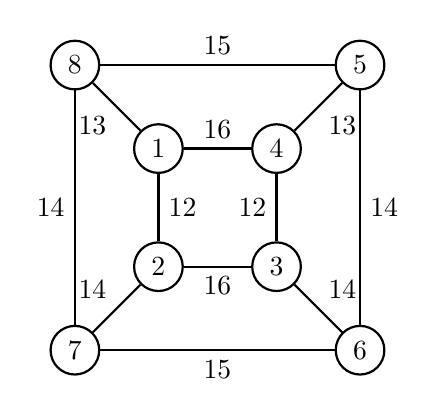
\begin{tikzpicture}[auto,node distance=1.5cm,
 thick,main node/.style={circle,draw}]
 
  \node[main node] (1) [] {1};
  \node[main node] (2) [below of=1] {2};
  \node[main node] (3) [right of=2] {3};
  \node[main node] (4) [above of=3] {4};
  \node[main node] (5) [above right of=4] {5};  
  \node[main node] (6) [below right of=3] {6};
  \node[main node] (7) [below left of=2] {7};
  \node[main node] (8) [above left of=1] {8};
  
  \foreach \s/\t/\i in {1/2/12, 1/4/16, 1/8/13, 3/2/16, 3/4/12, 3/6/14, 5/4/13, 5/6/14, 8/5/15, 7/2/14, 6/7/15, 7/8/14} {
   \path[draw] (\s) edge node {\i} (\t);}
\end{tikzpicture}
\end{center}
\column{.5\textwidth}
\begin{center}

\begin{tikzpicture}[auto,node distance=1.5cm,
 thick,main node/.style={circle,draw}]
 
  \node[main node] (1) [] {1};
  \node[main node] (2) [below of=1] {2};
  \node[main node] (3) [right of=2] {3};
  \node[main node] (4) [above of=3] {4};
  \node[main node] (5) [above right of=4] {5};  
  \node[main node] (6) [below right of=3] {6};
  \node[main node] (7) [below left of=2] {7};
  \node[main node] (8) [above left of=1] {8};
\only<2->{
  \foreach \s/\t/\i in {1/8/13} {
   \path[draw] (\s) edge node {\i} (\t);}
}
\only<3->{
  \foreach \s/\t/\i in {1/2/12} {
   \path[draw] (\s) edge node {\i} (\t);}
}
\only<4->{
  \foreach \s/\t/\i in {7/2/14} {
   \path[draw] (\s) edge node {\i} (\t);}
}
\only<5->{
  \foreach \s/\t/\i in { 6/7/15} {
   \path[draw] (\s) edge node {\i} (\t);}
}
\only<6->{
  \foreach \s/\t/\i in {3/6/14} {
   \path[draw] (\s) edge node {\i} (\t);}
}
\only<7->{
  \foreach \s/\t/\i in { 3/4/12} {
   \path[draw] (\s) edge node {\i} (\t);}
}
\only<8->{
  \foreach \s/\t/\i in {5/4/13} {
   \path[draw] (\s) edge node {\i} (\t);}
}	 
\end{tikzpicture}

\end{center}
\end{columns}

\end{frame}


%----------------------------------------------
\begin{frame}
\frametitle{Avoiding Cycles}
\begin{itemize}
\item How do we keep track of which nodes are in the MST and the shortest edge to add?
\item Use a adjacency list ($G$), and two dictionaries:
	\begin{itemize}
	\item $processed$ will map a node to a boolean, telling us if it is processed.
	\item $dist$ will map a node to its distance from the MST.
	\end{itemize}
\end{itemize}
\end{frame}
%---------------------------------------------
\begin{frame}
\frametitle{Prim's - Building the Dictionaries}
\begin{columns}[c]
\column{.5\textwidth}
\[
\begin{tabular}{|c|c|}
\multicolumn{2}{c}{$G$} \\
\hline
1 & (2, 12), (4, 16), (8,13)  \\
\hline 
2 & (1, 12), (3, 16), (7, 14) \\
\hline
3 & (2, 16), (4, 12), (6, 14) \\
\hline
4 & (1, 16), (3, 12), (5, 13) \\
\hline
5 & (4, 13), (6, 14), (8, 15) \\
\hline
6 & (3, 14), (5, 14), (7, 15) \\
\hline
7 & (2, 14), (6, 15), (8, 14) \\
\hline
8 &  (1, 13), (5, 15), (7, 14) \\
\hline
\end{tabular}
\]
\column{.25\textwidth}
\only<2->{
\[
\begin{tabular}{|c|c|}
\multicolumn{2}{c}{$processed$} \\
\hline
1 & false \\
\hline 
2 & false \\
\hline
3 & false \\
\hline
4 & false \\
\hline
5 & false \\
\hline
6 & false \\
\hline
7 & false \\
\hline
8 &  false \\
\hline
\end{tabular}
\]
}

\column{.25\textwidth}
\only<3->{
\[
\begin{tabular}{|c|c|}
\multicolumn{2}{c}{$dist$} \\
\hline
1 & $\infty$ \\
\hline 
2 & $\infty$ \\
\hline
3 & $\infty$ \\
\hline
4 & $\infty$ \\
\hline
5 & $\infty$ \\
\hline
6 & $\infty$ \\
\hline
7 & $\infty$ \\
\hline
8 & $\infty$ \\
\hline
\end{tabular}
\]
}
\end{columns}

\vspace{.5cm}

\only<1>{
First we have our adjacency list. Each node is mapped to a list of the nodes it is connected to, along with the weight of the edge.
}
\only<2>{
Next, $processed$ maps each node to a boolean, indicating whether it's in the MST or not. We start with all of them false.
}
\only<3>{
Last, $dist$ maps nodes to thier distances from the MST. To start, since there are no nodes in the MST, the distances are $\infty$.
}
\end{frame}
%---------------------------------------------
\begin{frame}
\frametitle{Prim's Algorithm Example}

\begin{columns}[c]
\column{.5\textwidth}
\[
\begin{tabular}{|c|c|}
\multicolumn{2}{c}{$G$} \\
\hline
\textbf<9-12>{1} & \textbf<10>{(2, 12)}, \textbf<11>{(4, 16)}, \textbf<12>{(8,13)}  \\
\hline 
\textbf<15-18>{2} & \textbf<16>{(1, 12)}, \textbf<17>{(3, 16)}, \textbf<18>{(7, 14)} \\
\hline
\textbf<38>{3} & \textbf<39>{(2, 16)}, \textbf<40>{(4, 12)}, \textbf<41>{(6, 14)} \\
\hline
\textbf<33>{4} & \textbf<34>{(1, 16)}, \textbf<35>{(3, 12)}, \textbf<36>{(5, 13)} \\
\hline
\textbf<27>{5} & \textbf<28>{(4, 13)}, \textbf<29>{(6, 14)}, \textbf<30>{(8, 15)} \\
\hline
6 & (3, 14), (5, 14), (7, 15) \\
\hline
\textbf<21>{7} & \textbf<22>{(2, 14)}, \textbf<23>{(6, 15)}, \textbf<24>{(8, 14)} \\
\hline
\textbf<3-6>{8} &  \textbf<4>{(1, 13)}, \textbf<5>{(5, 15)}, \textbf<6>{(7, 14)} \\
\hline
\end{tabular}
\]


	\column{.25\textwidth}
	\[
	\begin{tabular}{|c|c|}
	\multicolumn{2}{c}{$processed$} \\
	\hline
	1 & \only<1-7>{false}\only<8->{\textbf<8>{true}} \\
	\hline 
	2 & \only<1-13>{false}\only<14->{\textbf<14>{true}} \\
	\hline
	3 & \only<1-37>{false}\only<38->{\textbf<38>{true}} \\
	\hline
	4 & \only<1-31>{false}\only<32->{\textbf<32>{true}} \\
	\hline
	5 & \only<1-25>{false}\only<26->{\textbf<26>{true}} \\
	\hline
	6 & \only<1-42>{false}\only<43->{\textbf<43>{true}} \\
	\hline
	7 & \only<1-19>{false}\only<20->{\textbf<20>{true}} \\
	\hline
	8 &  \only<1>{false}\only<2->{\textbf<2>{true}} \\
	\hline
	\end{tabular}
	\]
	\column{.25\textwidth}
	\[
	\begin{tabular}{|c|c|}
	\multicolumn{2}{c}{$dist$} \\
	\hline
	\textbf<7>{1} & \only<1-3>{$\infty$}\only<4-7>{\textbf<4,7>{13}}\only<8->{\textbf<8,16,34>{0}} \\
	\hline 
	\textbf<13>{2} & \only<1-9>{$\infty$}\only<10-13>{\textbf<10,13>{12}}\only<14->{\textbf<14,22,39>{0}} \\
	\hline
	\textbf<37>{3} & \only<1-16>{$\infty$}\only<17-34>{\textbf<17>{16}}\only<35-37>{\textbf<35>{12}}\only<38->{\textbf<38>{0}} \\
	\hline
	\textbf<31>{4} & \only<1-10>{$\infty$}\only<11-27>{\textbf<11>{16}}\only<28-31>{\textbf<28>{13}}\only<32->{\textbf<32,40>{0}} \\
	\hline
	\textbf<25>{5} & \only<1-4>{$\infty$}\only<5-25>{\textbf<5>{15}}\only<26->{\textbf<26,36>{0}} \\
	\hline
	\textbf<42>{6} & \only<1-22>{$\infty$}\only<23-28>{\textbf<23>{15}}\only<29-42>{\textbf<29,41>{14}}\only<43->{\textbf<43>{0}} \\
	\hline
	\textbf<19>{7} & \only<1-5>{$\infty$}\only<6-19>{\textbf<6,18>{14}}\only<20->{\textbf<20>{0}} \\
	\hline
	8 & \only<1>{$\infty$}\only<2->{\textbf<2,12,24,30>{0}} \\
	\hline
	\end{tabular}
	\]
	\end{columns}
	
\begin{columns}[c]

\column{.5\textwidth}

\begin{itemize}
\only<1>{\item Start with our initialized dictionaries.}
\only<2>{\item Start at node 8. Change it's boolean in $processed$ to true and its distance to 0.}
\only<3-6>{\item Walk through 8's list of adjacent nodes and update their distances to the MST.}
\only <7-8,13-14,19-20, 25-26,31-32,37-38>{\item Add the node with the shortest distance to the MST. \only<1-14>{Add it to the list of nodes in the MST, change it's distance, and set it's boolean to true.}}
\only<9-11>{\item Walk through 1's neighbors and update their distances.}
\only<12>{\item 8 is already in the MST, so it's distance remains at 0.} 
\only<15-18>{\item Walk through 2's neighbors and update their distances.}
\only<21-24>{\item Walk through 7's neighbors and update their distances.}
\only<27-30>{\item Walk through 5's neighbors and update their distances.}
\only<33-36>{\item Walk through 4's neighbors and update their distances.}
\only<39-41>{\item Walk through 3's neighbors and update their distances.}
\only<42>{\item Add our last node to the MST and update $processed$ and $dist$.}
\only<43>{\item All nodes have now been processed, so we are done.}

\end{itemize}

\column{.5\textwidth}

\begin{center}
\begin{tikzpicture}[scale=.65, transform shape, auto,node distance=1.5cm,
 thick,main node/.style={circle,draw}]
 
  \node[main node] (1) [] {1};
  \node[main node] (2) [below of=1] {2};
  \node[main node] (3) [right of=2] {3};
  \node[main node] (4) [above of=3] {4};
  \node[main node] (5) [above right of=4] {5};  
  \node[main node] (6) [below right of=3] {6};
  \node[main node] (7) [below left of=2] {7};
  \node[main node] (8) [above left of=1] {8};
\only<7->{
  \foreach \s/\t/\i in {1/8/13} {
   \path[draw] (\s) edge node {\i} (\t);}
}
\only<14->{
  \foreach \s/\t/\i in {1/2/12} {
   \path[draw] (\s) edge node {\i} (\t);}
}
\only<20->{
  \foreach \s/\t/\i in {7/2/14} {
   \path[draw] (\s) edge node {\i} (\t);}
}
\only<26->{
  \foreach \s/\t/\i in { 8/5/15} {
   \path[draw] (\s) edge node {\i} (\t);}
}
\only<43->{
  \foreach \s/\t/\i in {3/6/14} {
   \path[draw] (\s) edge node {\i} (\t);}
}
\only<38->{
  \foreach \s/\t/\i in { 3/4/12} {
   \path[draw] (\s) edge node {\i} (\t);}
}
\only<32->{
  \foreach \s/\t/\i in {5/4/13} {
   \path[draw] (\s) edge node {\i} (\t);}
}	 
\end{tikzpicture}

\end{center}


\end{columns}
\end{frame}

%---------------------------------------------

%\begin{frame}
%\begin{algorithm}[H]
%\frametitle{Inserting an Edge into $shortest$}
%\begin{algorithmic}[1]
%\Procedure{InsertEdge}{$edge, shortest$}
%	\State Get the node that is reached by the edge
%	\If {$node$ is not in $processed$}
%		\State $shortest[node] \gets edge's value$
%	\Else
%		\State $shortest[node] \gets min(edge,shortest[node])$
%	\EndIf
%\EndProcedure
%\end{algorithmic}
%\end{algorithm}
%\end{frame}

%---------------------------------------------

\begin{frame}
\begin{algorithm}[H]
\frametitle{Prim's Algorithm - Pseudocode}
\begin{algorithmic}[1]
\Procedure{Prim}{$G,start$}
	\State$processed \gets$ a dictionary mapping every node to $false$ except for the nodes in $start$.
	\State $MST \gets $ empty list
	\State $shortest \gets$ a dictionary mapping every node to $\infty$.
	\State $shortest[start] \gets 0$
\While{$MST$ needs more nodes}
	\State $new \gets$ the shortest edge in $shortest$.
	\State $shortest[new] \gets 0$
	\State $MST \gets new$ 
	\State $processed[new] \gets true$
	\For {$n$ in $edges[new]$}
		\State $shortest[n] = min(n.value, shortest[n])$
	\EndFor
\EndWhile
\State \pseudoli{return} MST.
\EndProcedure
\end{algorithmic}
\end{algorithm}
\end{frame}


\end{document}